\documentclass[sigconf]{acmart}

\def\BibTeX{\textsc{Bib}\TeX}
\def\LaTeX{\textsc{La}\TeX}
\usepackage{url}
\usepackage{balance}
\usepackage{color}
\usepackage{enumerate}
\usepackage{listings}
\settopmatter{printacmref=false}

\setcopyright{none}
\renewcommand\footnotetextcopyrightpermission[1]{}
\pagestyle{plain}
\acmConference[CSCI]{}{Term Paper}{2021}

\begin{document}
\title{A Functional Genetic Algorithm for Knapsack Problems}

\author{Handong Chen \\  \href{mailto:hc2157@rit.edu}{hc2157@rit.edu}}

\begin{abstract}
Functional programming (FP) is robust, safe, and efficient because of its unique features. Although FP languages are pretty tricky for new programmers compared to OOP, they are still active in areas such as financial analysis, driver verification, industrial robot programming, and static analysis of embedded software.~\cite{paper1}
The unique mechanism of the genetic algorithm is from biology. It is a computation model that simulates creature evolution and genetics concepts. In other words, it is a method that can search for the optimal result by mimicking the natural evolution process. Because of its mechanism, the genetic algorithm has a higher possibility of finding the global optimal result than standard greedy algorithms. 

Because of the unique features of functional programming, we implemented a genetic algorithm with the functional programming style, specifically the language Haskell. Our algorithm uses rank-based selection, single-point crossover, and flip-bit mutation methods. We did a performance evaluation showing that the algorithm can effectively solve the Knapsack problem in the analysis part. We also got ideas from another paper~\cite{choosenPaper} that presented a generic genetic algorithm. Their higher-order function can be used in any genetic algorithm that helps us implement the genetic algorithm in FP style.
\end{abstract}

\keywords{Functional Programming, Genetic Algorithm, Knapsack Problem}

\maketitle

\section{Introduction}
\label{intro}

A genetic algorithm is a search heuristic algorithm based on Charles Darwin's natural selection hypothesis. This algorithm simulated natural evolution, in which the fittest individuals are chosen to create the next generation. It would repeat this process until it met the stopping criteria.

The selection of the fittest individuals from a population begins the natural selection process. They generate offspring who inherit the parents' qualities and are passed down to the next generation. If parents are physically active, their children will be fitter and have a better chance of surviving. This procedure will iterate until a generation of the fittest individuals is discovered. 

A standard genetic algorithm has five steps.
\begin{enumerate}
  	\item Initial population
  	\item Fitness function
  	\item Selection
	\item Crossover
	\item Mutation
\end{enumerate}

\begin{figure}
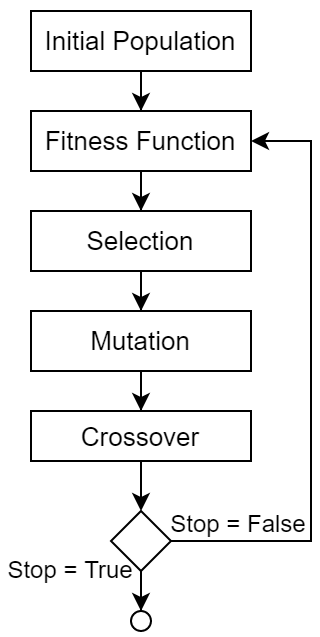
\includegraphics[scale=0.5]{GA Structure}
\caption{Genetic Algorithm Structure}
\end{figure}
The initial population is the first step. The procedure starts with a group of chromosomes known as a Population. Each chromosome is a potential solution to the problem. Gene is a binary number representing whether we will use the item. A chromosome is a string of genes. Also, we can consider it as a solution. 

The fitness function is an evaluation function that calculates the chromosome score. Depending on the selection methods, a fitness score may determine the probability of a chromosome going to the crossover process. For Knapsack problems, weight usually will be the fitness score of each individual. 

The selection process selects several pairs of individuals to be the parents and passes their genes to the next generation. There are multiple methods to choose a pair of individuals. In our project, we use the rank-based selection method. Furthermore, the research team used the tournament selection method in the general genetic algorithm. 

Crossover is one of the most essential processes in this type of algorithms. Crossover and mutation allowed genetic algorithms to find global optimal solutions rather than stuck at the local optimal result. Two parents will exchange their genes based on the crossover point in this process. Hence, the offspring will have part of both parents' genes. In our algorithm, we use a static single-point crossover. However, the general genetic algorithm uses random points to do the process.

The mutation is another important process. When new offspring are created, the mutation process will randomly change one or more genes in their chromosomes. Mutation occurs to maintain diversity within the population and prevent premature convergence.~\cite{paper2} We perform mutation to each gene in a chromosome. On the other hand, the general genetic algorithm did the same method.


\section{Related Work}
\label{related}
Selection, crossover, and mutation are the most important process in a genetic algorithm. All of them have multiple implementation methods. For the selection part, rank-based selection, roulette wheel selection, and stochastic universal sampling are the most common methods. Rank-based selection means randomly selecting k individuals from the population. Then select the individual with the highest fitness score. Roulette wheel selection means forming a wheel based on the fitness scores of all the individuals and selecting the individual at a certain point of the wheel. Stochastic universal sampling is very similar to the roulette wheel selection method. It will select individuals at multiple wheel points rather than only one point. 

Crossover has seven methods, single-point, two-point, k-point, uniform, ordered, blend, and simulated binary crossover. The most common methods are single-point crossover and k-point crossover. In addition, the single-point crossover also can be considered as a k-point crossover when k is equal to 1. K-point crossover means randomly selecting multiple points on the genes and exchanging the genes between two parents. Finally, the children will have genes from both parents, but only part of them. This method can improve the possibility of the algorithm to find a better global optimal solution to the problem.

Mutation has five methods, flip bit mutation, swap mutation, inversion mutation, scramble mutation, and real mutation. Flip bit mutation and swap mutation are the most common methods for this process. Flip bit mutation means one or more genes in the chromosome will randomly change. For example, a chromosome "110111" may become "110110". Swap mutation means one random pair of genes in the chromosome exchange their position. For example, a chromosome "123456" may become "163452".

\section{Implementation}
\label{Implementation}

\subsection{Populations}
A population is a set of chromosomes, and we use string to represent a chromosome. In our algorithm, the content of the string will be a list of binary numbers. 
\begin{lstlisting}
type Chromosome = String
type Population = [Chromosome]
\end{lstlisting}

\subsection{Fitness}
A fitness function is a function that can calculate the fitness score based on the genes in the chromosome and the meaning of each gene. We use the Int data type to represent the fitness score. In order to make the code simple, we use a pair of chromosomes and fitness scores to do the later computation. 
\begin{lstlisting}
type Fitness = Int
type ChromosomeF = (Chromosome, Fitness)
fitnessCal :: [String] -> Int -> 
              [(Int, Int)] -> [ChromosomeF]
 \end{lstlisting}

\subsection{Initial Populations}
In this part, we convert the base population from the input data to a list of ChromosomeF. All the chromosomes will be assigned a fitness score during the process to help the later computation. The implementation is pretty straightforward. The code will traverse all the genes in a chromosome and all the item data simultaneously to calculate the sum of scores. 
\begin{lstlisting}
initialPopulation :: Population -> Int -> 
                     [(Int, Int)] -> 
                     [ChromosomeF]
\end{lstlisting}

\subsection{Selection}
Our selection function will take four Int parameters and a list of ChromosomeF. These parameters represent the length of a chromosome, the seed of random functions, the number of selected elements, and the number of pairs. We use the rank-based selection method in the algorithm. The selection function will randomly choose n pairs of individuals from the population and only choose one individual with the highest fitness score from one pair.
\begin{lstlisting}
select :: Int -> Int -> Int -> 
          Int -> [ChromosomeF] -> 
          [(Chromosome, Chromosome)]
\end{lstlisting}

\subsection{Crossover}
The crossover function will take a pair of parents' chromosomes and do a single-point crossover. Finally, return a pair of children's chromosomes. The algorithm will exchange the genes from the middle point of the chromosome. 
\begin{lstlisting}
crossover :: (Chromosome, Chromosome) -> 
             (Chromosome, Chromosome)
\end{lstlisting}
\subsection{Mutation}
The mutation function is a traverse function. It will traverse all the genes in a chromosome and perform flip bit mutation methods to each gene. The mutation function takes a chromosome, a float number representing the mutation possibility, and an Int seed number. 
\begin{lstlisting}
mutation :: Chromosome -> Float -> 
            Int -> Chromosome
\end{lstlisting}
\section{Analysis}
\label{analysis}
Our test case is a simple Knapsack problem. The input data are six pairs of Int numbers. The first number of the pair represents the item's weight. The second number represents the item's fitness score. 

\[[(15, 15), (3, 7), (2, 10), (5, 5), (9, 8), (20, 17)]\]

Our test case shows that the standard genetic algorithm may throw previous good solutions and generate worse solutions. Hence, we added a variable to record the current best solution. Finally, the test case can be solved in 25 generations. The detailed information is shown in figure 2. 
\begin{figure}
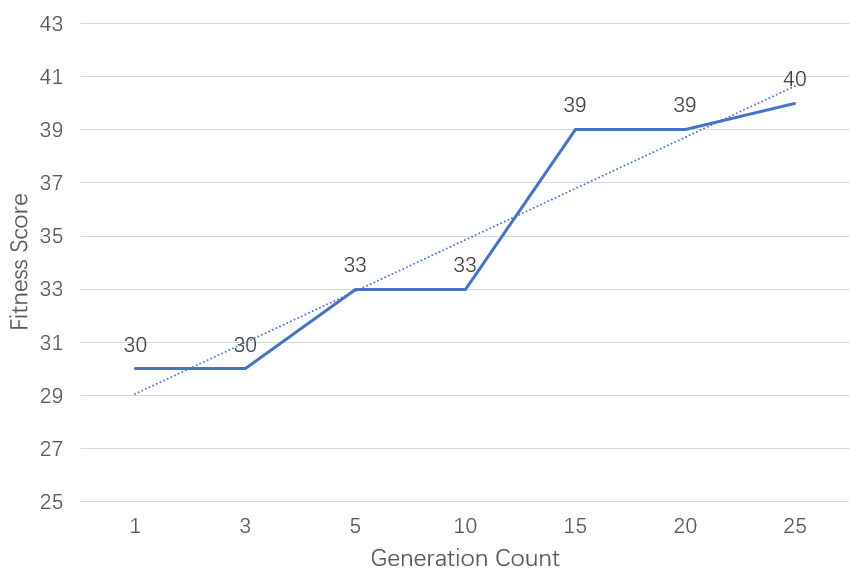
\includegraphics[scale=0.35]{Test Result}
\caption{Test Result}
\end{figure}

\subsection{Difference}
The general genetic algorithm~\cite{choosenPaper} has a similar structure to our algorithm. Their algorithm also uses the rank-based selection method. However, for the mutation process, they used a swap method. Also, they combined a random function for the crossover function to allow more randomness in this process. However, the general algorithm has a general function that can compile different input data to the same form of data. Then the algorithm will generate a random population and start the computation. Hence their algorithm can be used in almost any problem that a genetic algorithm can solve. In the paper, the research team represents their performance evaluation in bin packing problem, traveling salesPerson, and N-queens problem. 

\section{Conclusions}
\label{conclusions}

We presented a standard genetic algorithm implemented in a functional programming style. This algorithm used rank-based selection, single-point crossover, and flip-bit mutation methods. This algorithm can solve the Knapsack problem. We also did a performance test in the analysis selection. The result shows that the algorithm can solve this problem in a reasonable amount of time. We got the idea from another paper~\cite{choosenPaper}. Their research team presented a general genetic algorithm that can solve any problem solvable by a genetic algorithm. Moreover, in the analysis section, we also analyzed the difference between our algorithm and the general algorithm. We should implement more variant methods for selection, crossover, and mutation processes for future work. In addition, the algorithm should be implemented in a more general way and tested with more problems in the future. 



\balance
\bibliographystyle{ACM-Reference-Format}
\bibliography{researchpaper} 

\end{document}
